%% This is file `sample-acmsmall.tex',
%% generated with the docstrip utility.
%%
%% The original source files were:
%%
%% samples.dtx  (with options: `acmsmall')
%% 
%% IMPORTANT NOTICE:
%% 
%% For the copyright see the source file.
%% 
%% Any modified versions of this file must be renamed
%% with new filenames distinct from sample-acmsmall.tex.
%% 
%% For distribution of the original source see the terms
%% for copying and modification in the file samples.dtx.
%% 
%% This generated file may be distributed as long as the
%% original source files, as listed above, are part of the
%% same distribution. (The sources need not necessarily be
%% in the same archive or directory.)
%%
%%
%% Commands for TeXCount
%TC:macro \cite [option:text,text]
%TC:macro \citep [option:text,text]
%TC:macro \citet [option:text,text]
%TC:envir table 0 1
%TC:envir table* 0 1
%TC:envir tabular [ignore] word
%TC:envir displaymath 0 word
%TC:envir math 0 word
%TC:envir comment 0 0
%%
%%
%% The first command in your LaTeX source must be the \documentclass
%% command.
%%
%% For submission and review of your manuscript please change the
%% command to \documentclass[manuscript, screen, review]{acmart}.
%%
%% When submitting camera ready or to TAPS, please change the command
%% to \documentclass[sigconf]{acmart} or whichever template is required
%% for your publication.
%%
%%
% \documentclass[acmsmall]{acmart}
\documentclass[acmsmall,manuscript, screen, review]{acmart}
% \documentclass[acmsmall]{acmart}
% \usepackage{ragged2e} % don't use it
% \usepackage{bigstrut} % don't use
\usepackage{multirow}
\usepackage{float} 
\usepackage{subcaption}
 

%%
%% \BibTeX command to typeset BibTeX logo in the docs
\AtBeginDocument{%
  \providecommand\BibTeX{{%
    Bib\TeX}}}

%% Rights management information.  This information is sent to you
%% when you complete the rights form.  These commands have SAMPLE
%% values in them; it is your responsibility as an author to replace
%% the commands and values with those provided to you when you
%% complete the rights form.
\setcopyright{acmcopyright}
\copyrightyear{2018}
\acmYear{2018}
\acmDOI{XXXXXXX.XXXXXXX}


%%
%% These commands are for a JOURNAL article.
\acmJournal{JACM}
\acmVolume{37}
\acmNumber{4}
\acmArticle{111}
\acmMonth{8}

%%
%% Submission ID.
%% Use this when submitting an article to a sponsored event. You'll
%% receive a unique submission ID from the organizers
%% of the event, and this ID should be used as the parameter to this command.
%%\acmSubmissionID{123-A56-BU3}

%%
%% For managing citations, it is recommended to use bibliography
%% files in BibTeX format.
%%
%% You can then either use BibTeX with the ACM-Reference-Format style,
%% or BibLaTeX with the acmnumeric or acmauthoryear sytles, that include
%% support for advanced citation of software artefact from the
%% biblatex-software package, also separately available on CTAN.
%%
%% Look at the sample-*-biblatex.tex files for templates showcasing
%% the biblatex styles.
%%

%%
%% The majority of ACM publications use numbered citations and
%% references.  The command \citestyle{authoryear} switches to the
%% "author year" style.
%%
%% If you are preparing content for an event
%% sponsored by ACM SIGGRAPH, you must use the "author year" style of
%% citations and references.
%% Uncommenting
%% the next command will enable that style.
%%\citestyle{acmauthoryear}


%%
%% end of the preamble, start of the body of the document source.
\begin{document}

%%
%% The "title" command has an optional parameter,
%% allowing the author to define a "short title" to be used in page headers.
\title{ViST: A Ubiquitous Model with Multimodal Fusion for Crop Growth Prediction}

%%
%% The "author" command and its associated commands are used to define
%% the authors and their affiliations.
%% Of note is the shared affiliation of the first two authors, and the
%% "authornote" and "authornotemark" commands
%% used to denote shared contribution to the research.
\author{Junsheng Li}
% \authornote{Both authors contributed equally to this research.}
\email{22s103187@stu.hit.edu.cn}
\orcid{0000-0002-7724-7787}
% \authornotemark[1]

\affiliation{%
  \institution{Department of Computer Science and Technology, Harbin Institute of Technology}
  \streetaddress{No. 92, Xidazhi Street, Nangang District}
  \city{Harbin}
  \state{Heilongjiang Province}
  \country{China}
  \postcode{150000}
}

\author{Ling Wang}
\email{wangling@hit.edu.cn}
\affiliation{%
  \institution{Department of Computer Science and Technology,Harbin Institute of Technology}
  \streetaddress{No. 92, Xidazhi Street, Nangang District}
  \city{Harbin}
  \state{Heilongjiang Province}
  \country{China}
  \postcode{150000}
}


\author{Jie Liu}
\email{jieliu@hit.edu.cn}
\affiliation{%
  \institution{Department of Computer Science and Technology,Harbin Institute of Technology}
  \streetaddress{No. 92, Xidazhi Street, Nangang District}
  \city{Harbin}
  \state{Heilongjiang Province}
  \country{China}
  \postcode{150000}
}

\author{Jinshan Tang}
\email{jtang25@gmu.edu}
\affiliation{%
  \institution{Health Informatics, College of Public Health,George Mason University}
  \city{Fairfax}
  \state{VA}
  \country{USA}
  \postcode{22033}
}

%%
%% By default, the full list of authors will be used in the page
%% headers. Often, this list is too long, and will overlap
%% other information printed in the page headers. This command allows
%% the author to define a more concise list
%% of authors' names for this purpose.
\renewcommand{\shortauthors}{Junsheng et al.} % 页眉右上角

%%
%% The abstract is a short summary of the work to be presented in the
%% article.
\begin{abstract}
  Crop growth prediction can help agricultural workers to make accurate and reasonable decisions on farming activities. Existing crop growth prediction models focus on one crop and train a single model for each crop. In this paper, we will develop a ubiquitous growth prediction model for multiple crops, aiming to train a single model for multiple crops. A ubiquitous vision and sensor transformer(ViST) model for crop growth prediction with image and sensor data is developed to achieve the goals. In the proposed model, a cross-attention mechanism is proposed to implement the fusion of multimodal feature maps to reduce the computational cost and balance the interactive effects between features. For training the model, we combine the data from multiple crops to train a single (ViST) model. A sensor network system is constructed for the data collection on the farm that plants rice, soybean, and maize. Experiment results show that the proposed ViST model has an excellent ubiquitous ability for crop growth prediction with multiple crops.
\end{abstract}

%%
%% The code below is generated by the tool at http://dl.acm.org/ccs.cfm.
%% Please copy and paste the code instead of the example below.
%%
\begin{CCSXML}
  <ccs2012>
  <concept>
  <concept_id>10010147.10010178</concept_id>
  <concept_desc>Computing methodologies~Artificial intelligence</concept_desc>
  <concept_significance>500</concept_significance>
  </concept>
  </ccs2012>
\end{CCSXML}

\ccsdesc[500]{Computing methodologies~Artificial intelligence}

%%
%% Keywords. The author(s) should pick words that accurately describe
%% the work being presented. Separate the keywords with commas.

\keywords{crop growth prediction,ubiquitous model, multimodal learning, transformer module,cross-attention mechanism}

\received{20 February 2007}
\received[revised]{12 March 2009}
\received[accepted]{5 June 2009}

%%
%% This command processes the author and affiliation and title
%% information and builds the first part of the formatted document.
\maketitle

\section{Introduction}
With the development of new technologies such as the Internet of things, big data, and artificial intelligence (AI), modern agriculture has been dramatically changed. One major task in modern agriculture is to predict crop growth. Crop growth prediction is used as the weather vane for agricultural activities. Accurate short-range prediction of crop growth can help farmers manage fertilization, irrigation, and pesticide spraying effectively. With the effective management of these agricultural activities, human and material resources can be reduced as much as possible, and the final yields and economic benefits can be significantly improved. It can also reduce the use of pesticides that pollute the environment and thus protect the ecological environment.

There are many existing crop models for crop growth and yield prediction \cite{book,BRISSON2003309,boogaard1998wofost}. However, these models are designed for a specific crop and specific region and condition, which are not ubiquitous models. These models cannot be adaptive to any specific crop in different regions. The parameters and driving variables of the models are derived from the situation of a particular location, which can be measured and available under ideal conditions. Due to the inherent soil heterogeneity and the influence of farming methods on soil properties, the measured parameters will also be different. Because the biological system is too complex and many processes involved have to be fully understood, a ubiquitous model based on biology is different to build. A data-driven model with Neural Network makes it possible to build a ubiquitous model. Under the deep learning model, any dynamic systems, including crop systems, can be approximated through network structure design \cite{lecun_deep_2015,2020Deep}.

In the past, much research has focused on multi-scale crop images collected by UAV or satellite remote sensing for crop growth and yield prediction \cite{wang_new_2022,yue_estimate_2019,turkoglu_crop_2021}. These image data reflect the phenotype characteristics of crops. The dynamic changes of crop phenotypes, such as the Leaf Area Index, predict crop growth for a large region. Some researchers combine crop spectral data and soil and meteorological data for crop growth prediction \cite{trnka_effect_2007,islam_deep_2018,adisa_application_2019,liu_neural_2001,matsumura_maize_2015}. However, these data-driven methods still need to be ubiquitous. The results are strongly related to collecting high-precision crop parameters and input data of crop environment. The data collection processing is costly, hardly leading to the use for farm management. The leaf area index (LAI) is a comprehensive index related to individual and group characteristics of crop growth \cite{__1999}. The leaf area index (LAI) is selected as an prediction index of crop growth. LAI cannot reflect all individual and group characteristics and must be supplemented by ground monitoring \cite{carlson_relation_1997}. Since images and sensors can provide adequate information on crop growth, images and sensors can be used as supplements to ground monitoring. 

To approximate the objective function, a model has to be built to apply to multimodal and multi-dimension data. Most existing multimodal mechanisms exist in automotive drive and medical fields \cite{guo2019deep, xiao2020multimodal}. Our work is the first to fuse crop RGB image and sensor data for low-cost crop growth prediction on farms. The multimodal fusion process fuses information from two or more modalities to realize information complementation and broaden the coverage of information contained in the input data. Different from other fields, the estimation model for crop growth by multimodal fusion has more challenges in generalization as each crop has its character. To solve this problem, we propose the ViST (Vision and Sensor Transformer) model, which can realize efficient information fusion for accurate prediction of crop growth.

Besides the fusion of multiple data resources for crop growth, we also investigate the possibility of hybrid training, which aims at developing a single network to predict the crop growth of multiple crops. In the past, many models for crop growth prediction were developed. However, all of these models were trained using a single crop, which means each crop needs a single model. On a farm, there are generally many crops. Training is time-consuming and complex for farmers if each crop needs a trained model. Thus, this paper aims to develop a ubiquitous model that could be used for multiple crops. A sensor network system is constructed for the data collection on the farm that plants rice, soybean, and maize.

The main contributions of this paper are as follows:

•	We proposed a ViST (Vision and Sensor Transformer) model for crop growth, which can efficiently utilize a multimodal data fusion mechanism. 

•	We also investigated the possibility of hybrid training, which aims at developing a single network to predict crop growth of multiple crops.  

•	The proposed model was compared with other existing models using data from farms we collected, and the proposed model can obtain better performance than other current models.





\section{Related Work}
\subsection{Single-modality approaches for crop growth prediction}
Single-modality approaches for crop growth prediction include two types of methods: image-only and non-image sensor-only strategies. Image-based remote sensing technology for crop growth prediction is one of the image-only approaches. Image-based remote sensing technology has attracted attention as it can estimate crop growth effectively due to its ability to provide timely, dynamic, and macro-scale observations \cite{__2016}. With the development of machine learning techniques, image-based remote sensing technology for crop growth has developed further. They are often combined with machine learning techniques to estimate crop growth \cite{johnson_crop_2016,zhong_deep_2019,yang_deep_2019}. However, the quality of images acquired through traditional remote sensing is often affected by weather and cloud changes and thus affects the prediction. Besides, remote sensing technology generally has high maintenance and operation costs, affecting its vast uses. Recently, convenient image-based techniques based on UAV drew the researchers’ attention \cite{weiss_plant_2011,tao_estimation_2020,zhou_predicting_2017,maimaitijiang_unmanned_2017,wan_grain_2020}. By mounting a camera to a UAV, high spatial resolution images of crops can be acquired and thus can be used for crop growth estimation. These techniques are beneficial for small farms.

Non-image sensor-only approaches are also popular for growth prediction. Because crop growth is affected by climate/weather and soil conditions \cite{fortin_site-specific_2011,campbell_effect_1988,ehret_neural_2011}, thus meteorological and soil sensors have been widely used to predict crop growth attributes. These non-image sensor-only approaches often use machine learning techniques. Dahikar et al. \cite{dahikar_agricultural_2014} proposed a crop prediction method by sensing various soil parameters and parameters related to the atmosphere and using ANN for crop yield prediction in rural areas. O'Neal et al. \cite{oneal_neural_2002} designed a fully connected network to predict maize yield using local crop stage weather data and yield data from 1901 to 1996. Morimoto et al. \cite{morimoto_dynamic_2007} used a deep learning model to identify changes in citrus sugar and citric acid content based on rainfall and sunshine duration data. Drummond et al. \cite{drummond_application_1998} applied feedforward neural networks to estimate nonlinear relationships between soil parameters and crop yields. Kitchen et al. \cite{kitchen_soil_2003} found that neural networks could provide the most accurate empirical model of the data and fit the yield data well to soil and terrain features.





\subsection{Multimodal learning for crop growth prediction}
Image-only and non-image sensor-only approaches have shown impressive results in predicting crop growth \cite{padilla_proximal_2018}. However, regarding the integrity of information expression, the model obtained by a single modality still has certain defects for missing information. One solution is to integrate the representations of these two modalities to take advantage of their complementary advantages in crop growth prediction.

Many deep learning-based approaches have been developed to handle multimodal data \cite{sengupta_review_2020, 8269806, liang_foundations_2023}. Multimodal machine learning has led to a wide range of applications: from audiovisual speech recognition (AVSR)\cite{yuhas_integration_1989}, multimedia content indexing and retrieval \cite{snoek_multimodal_2005}, understanding human multimodal behavior, multimodal emotion recognition \cite{chen_heu_2021}, image and video captioning \cite{lei_video_2021}, VQA\cite{long_improving_2021}, multimedia retrieval \cite{souza_online_2021}, to health analytics \cite{yazdavar_multimodal_2020}, etc. Huang et al. \cite{huang_what_2021} proved from a theoretical point of view that multimodal learning could fuse the information of single modalities and complement each other so that the final effect of the model is better than that of a single modality.

 In agriculture, there is some research on multimodal learning. Dang et al. \cite{dang2021autumn} used DNN with a multilayer feedforward perceptron(MLP) model for crop yield prediction. Chu et al. \cite{chu_end--end_2020} proposed an end-to-end prediction model for summer and winter rice yield based on MLP deep learning fusion. Two simple MLPS were used to extract spatial and temporal features, and then these two simple MLP models were combined to mine the relationship between features and rice yield. The model maintained stable convergence after 100 iterations. Maimaitijiang et al. \cite{maimaitijiang_soybean_2020} tried to use multimodal data fusion to complete tasks related to crop growth. The combined multimodal information, such as canopy spectral, structural, thermal, and texture features, are extracted. Input-level and middle-level feature fusion by MLP are used to predict crop grain yield.

However, the previous work uses MLP for data fusion in the NN models. The problem is that it is suitable for small-scale learning. When the model scale is enlarged, it will suffer from serious overfitting. Due to extensive data in images, it is difficult for MLP to extract features efficiently \cite{zhao_battle_2021}. In addition, the learning efficiency of fully connected architectures is very low, which has long been confirmed by machine learning experiments. Inefficiency means that more training data are needed to reach a certain level of performance. Many application scenarios cannot provide enough data support, so it is necessary to introduce assumptions to improve the utilization efficiency of limited data. Therefore, the application scenarios of the fully connected architecture are limited, and there are also problems of poor interpretability and robustness.

With the success of Transformers and self-supervised learning, there has been increasing research on cross-modal learning, such as vision-language pre-trained models (VLP)\cite{clevers_remote_2013}, images and lidar fusion\cite{prakash_multi-modal_2021}, Audio set, Epic-Kitchens, and VGGSound classification \cite{nagrani_attention_nodate}. The attention adaptively generated by Transformer has good adaptability. Attention can filter out a small amount of important information from a large amount of data, focus on this vital information, and ignore the most unimportant information. The information is critical, and more weight can be assigned. That is, the weight represents the importance of the data \cite{vaswani_attention_2017}.

The multimodal fusion process fuses information from two or more modalities to realize information complementation and broaden the coverage of information contained in the input data. \cite{ 8269806} However, it inevitably adds much redundant information. Therefore, a more effective way of information fusion and expression is needed.

 




A multimodal learning method based on Transformer\cite{vaswani_attention_2017} is proposed to complete the task of crop growth prediction. Compared with MLP \cite{ maimaitijiang_soybean_2020}, Transformer can extract features efficiently on tasks with a large amount of data, such as images and sensors. As a result, unnecessary calculations are reduced, and the efficiency and robustness of the prediction model are improved. The modular structure of the Transformer model allows for flexible processing of different types of inputs. Different types of features can be inputted into different modules of the Transformer and combined for further processing. This structure makes it easier to expand the model to accommodate different types of data, facilitating the fusion of multimodal data.

A cross-attention mechanism is proposed for fusing agricultural sensor and image data with fewer redundancy calculations. Besides, there are significant differences between the representations and feature spaces of images and sensor data. By using cross-attention mechanisms, images and sensor data can be jointly encoded and effectively complemented based on their common features. This enables the model to handle multimodal data better.


\section{Vision-and-Sensor Transformer model}

The proposed ViST overall network structure is shown in Figure \ref{model_structure}. The inputs are crop images and sensor data. In the framework, the MLP module and Linear Projection Flattened Patches module(LPFP) extract features from sensor and image data, respectively. LPFP was introduced by ViT\cite{dosovitskiy_image_2021}. The transformer encoder is designed for data fusion. Pooler and Linear modules are intended to reduce the dimension of features. The specific details of each module in the framework are described below.


\begin{figure}[htbp]
  \centering
  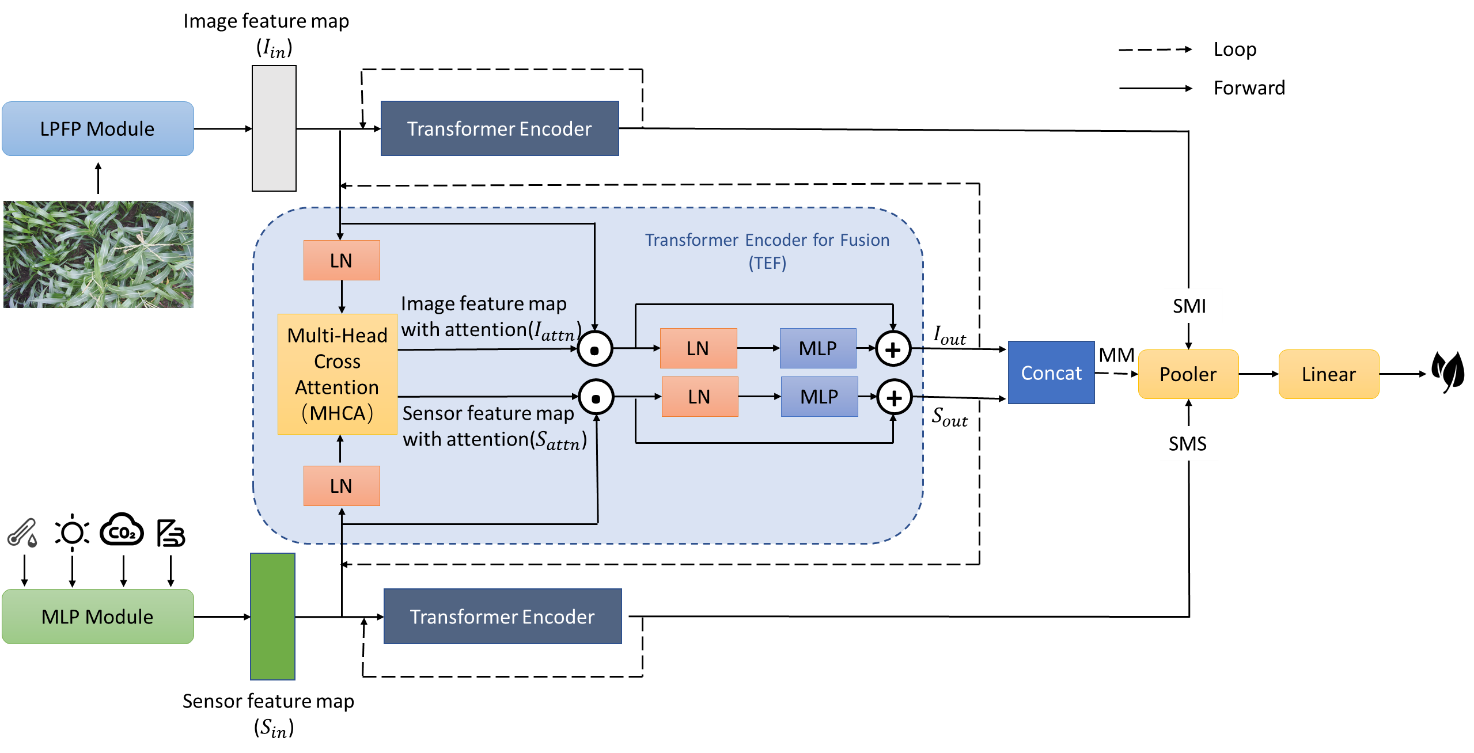
\includegraphics[width=\linewidth]{pic/model_structure.png}
  \caption{The framework of ViST for growth prediction. Solid lines represent forward and dashed lines represent loop. The input of the ViST is sensor and image data. They are processed independently at MLP and LPFP modules, respectively. The features from the two modules are input to one Transformer Encoder for feature fusion. The encoder output is given to the Concat module with the output for Multiple Modalities (MM). At the same time, the features are sent separately to the other two Transformer encoders for self-attention mechanics. The outputs of these two transformer encoders are Single Modality with Image(SMI) and Single Modal with Sensor(SMS). The results of MM, SMI, and SMS are then input into the Pooler module to reduce the dimension of the features. Finally, the features are input to the linear layer module to output the leaf area index (LAI) value (in the range of [0,1]).}
  \label{model_structure}
\end{figure}



\subsection{MLP Module}
Generally speaking, image data has three channels for RGB, and each pixel has a value. But sensor data only has dozens of values. Therefore, the number of values for Sensor data is much less than those for image data. Image data will dominate if the two data types are directly integrated; Simultaneously, the sensor data will not be well expressed.

To solve this problem, sensor data was converted into feature maps. MLP module can amplify the characteristics of the sensor data. The sensor data are composed of weather data and soil data. The data are numerical and have 19 data items. After data preprocessing, the sensor data were arranged into one-dimensional vectors and input into the multilayer feedforward perceptron(MLP) module. The specific structure of the MLP module is shown in Figure \ref{mlp_module}.


\begin{figure}[htbp]
  \centering
  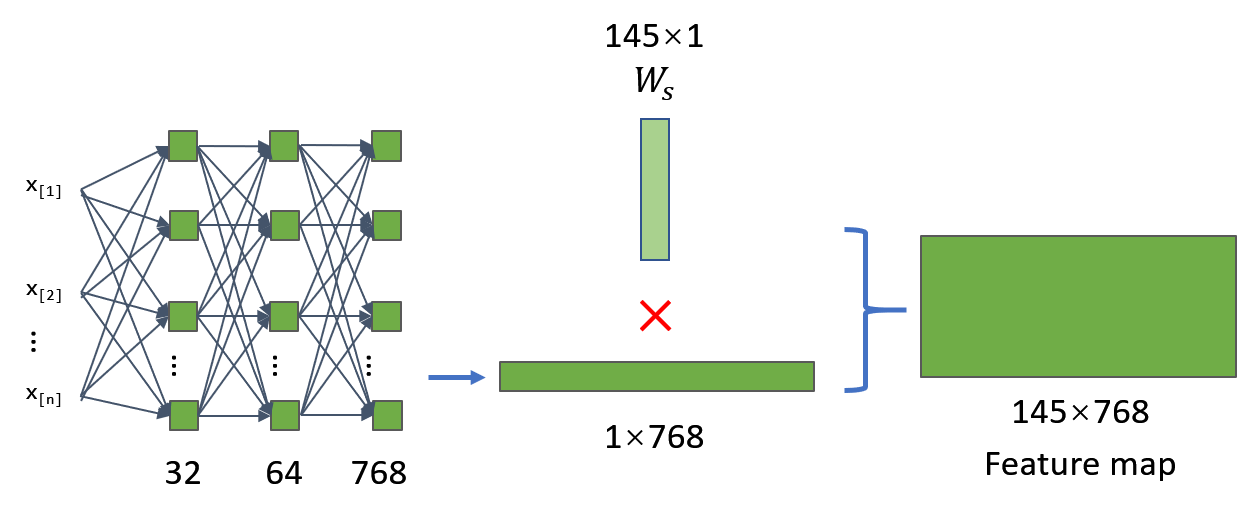
\includegraphics[width=0.7\linewidth]{pic/mlp_module.png}
  \caption{Sensor input model structure. The MLP module is a multilayer perceptron. It has 19 neurons at the input layer and 768 neurons at the output layer. The two hidden layers contain 32 and 64 neurons, respectively. We found the performance using 2-layer MLP and 3-layer MLP doesn’t have significant difference, thus we used the simpler 2-layer MLP.}
  \Description{Image and sensor input model structure.}
  \label{mlp_module}
\end{figure}
Following the output of the MLP module, a one-dimensional vector containing 768 elements is generated, resulting in a vector size of 1\begin{math}
  \times
\end{math}768. This vector is then transformed into a 145\begin{math}
  \times
\end{math}768 matrix using the following equation:


\begin{equation}
  M_{out}=W_s\times M_{in}
\end{equation}

where  \begin{math}   M_{in} \end{math}  refers to the 1x768 vector generated by the MLP module, which is then transformed into a 145\begin{math}
  \times
\end{math}768 matrix, denoted as \begin{math}
  M_{out}
\end{math}. \begin{math}
  W_s
\end{math} is a 145x1 matrix whose elements are obtained through training the model.

\subsection{Linear Projection Flattened Patches module}
In this paper, the sensor data is mapped to the same dimension as the image features of the LPFP module to facilitate subsequent feature fusion operations. It is worth noting that the sensor features based on the MLP module do not require position information, and the input order of sensor data can be arbitrarily scrambled.

\begin{figure}[htbp]
  \centering
  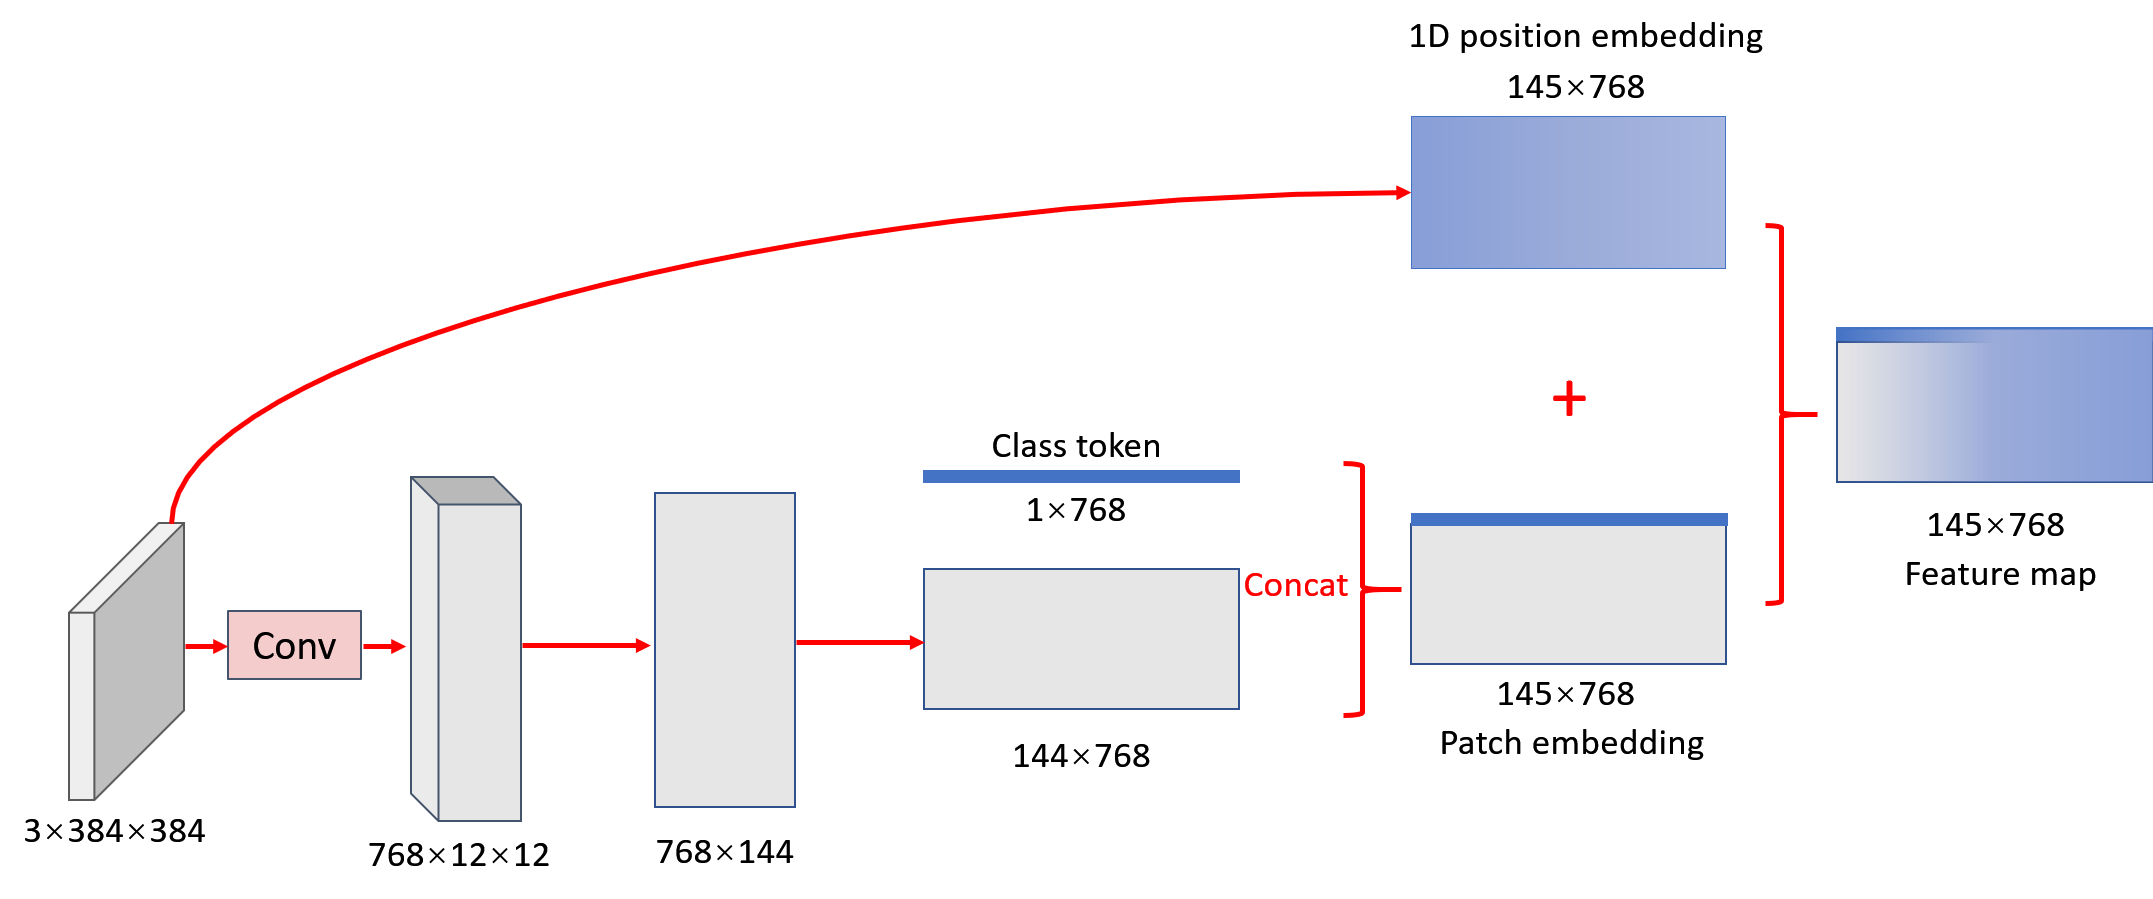
\includegraphics[width=\linewidth]{pic/linear_projection_flattened_patches_module.png}
  \caption{Linear Projection Flattened Patches module. Linear Projection Flattened Patches divide the image into several equal small images and align the image feature map with the sensor features through matrix transformation.}
  \Description{Create image feature.}
  \label{linear_projection}
\end{figure}

The structure of the linear projection flattened patches module is shown in Figure \ref{linear_projection}. The input of the module is an image with a size of CHANEL×HEIGHT×WIDTH (C×H×W). The 3D tensor corresponds to an RGB image. Before inputting the image, the image is adjusted to the size of 3×384×384, as shown in the input in Figure \ref{linear_projection}. The image is divided into 768 blocks with the size of 12×12 by convolution operation. The convolution operation was performed using a kernel of size 32×32. The stride of the convolution operation is 32. Each small image is flattened into 144 one-dimensional vectors, and 768 flattened one-dimensional vectors are successively connected into 768×144 vectors. The 768×144 vector is transposed to the 144×768 vectors to be fused with the feature vector from the sensor. Then, the 144×768 feature vector is concatenated with the class token vector to generate patch embedding. 

The Class Token is a specialized token that can represent the category information of an image. It is a vector that is typically added to the embedded representation of the image. The Class Token can provide additional information by encoding some global features that are shared by all images, which can help the model better understand the content of the images.

The position information of 1D Position embedding is added to patch embedding to retain positional information. Both class token and 1D Position embedding refer to ViT \cite{dosovitskiy_image_2021}. The position information of each pixel in an image can be transformed into a high-dimensional vector, where each dimension of the vector represents the position of the pixel in a specific dimension of the image. This high-dimensional vector can be concatenated with the feature vector of each pixel (e.g., color information, texture information, etc.), resulting in a higher-dimensional feature vector. ViT has proved that the performance of 2D position embedding is not better than that of 1D position embedding, so 1D position embedding is chosen. 

Finally, the Patch embedding is added to the 1D position embedding to obtain the feature map of the image.

The features of the image and the sensor are represented using vectors with the same dimensions. The vectors are ready to be input to the next transformer encoder for complete feature fusion.



\subsection{Transformer Encoder for fusion}
\begin{figure}[htbp]
  \centering
  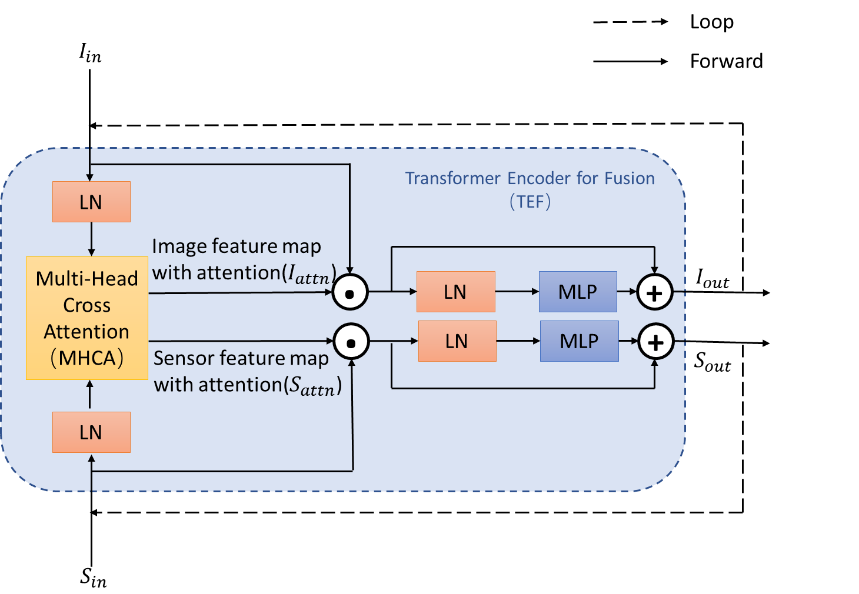
\includegraphics[width=0.8\linewidth]{pic/model_structure_TEF.png}
  \caption{The structure of the Transformer Encoder for Fusion (TEF) model consists of alternating layers of Multi-Head Cross Attention (MHCA), multiple layer perceptron (MLP) and Layer Normalization (LN) modules. MHCA is the central module responsible for fusing the image and sensor features. The MLP is adopted from ViT, and the LN module is responsible for performing Layer Normalization operations.}
  \Description{The structure of the Transformer Encoder for Fusion (TEF).}
  \label{model_structure_TEF}
\end{figure}




The Transformer Encoder for Fusion (TEF) model serves as the central model for multi-modal data fusion. The calculation process for TEF in Figure \ref{model_structure_TEF} is given as follows.


\begin{equation}
  I_{attn},S_{attn}=MHCA\left(I_{in},S_{in}\right)
\end{equation}
\begin{equation}
  I_{out}=MLP\left(LN\left(I_{in}\cdot I_{attn}\right)\right)+I_{in}\cdot I_{attn}
\end{equation}
\begin{equation}
  S_{out}=MLP\left(LN\left(S_{in}\cdot S_{attn}\right)\right)+S_{in}\cdot S_{attn}
\end{equation}

Here \begin{math}
  I_{attn}
\end{math} and \begin{math}
  S_{attn}
\end{math} are defined as the output of MHCA module, respectively. \begin{math}
  I_{attn}
\end{math},\begin{math}
  S_{attn}
\end{math} are Image and Sensor Feature Map with attention, respectively. \begin{math}
  I_{in}
\end{math},\begin{math}
  S_{in}
\end{math} are defined as the inputs of TEF, respectively. \begin{math}
  I_{out}
\end{math} and \begin{math}
  S_{out}
\end{math} are outputs of TEF, respectively. \begin{math}
  I_{in}
\end{math} and \begin{math}
  I_{out}
\end{math} are Image Feature Maps. \begin{math}
  S_{in}
\end{math} and \begin{math}
  S_{out}
\end{math} are Sensor Feature Maps. There are 12 loop computations for TEF. The output of TEF \begin{math}
  I_{out}
\end{math} and \begin{math}
  S_{out}
\end{math} are the input for TEF at next loop. After 12 loops is finished, \begin{math}
  I_{out}
\end{math} and \begin{math}
  S_{out}
\end{math} are given to next module.

\begin{figure}[htbp]
  \centering
  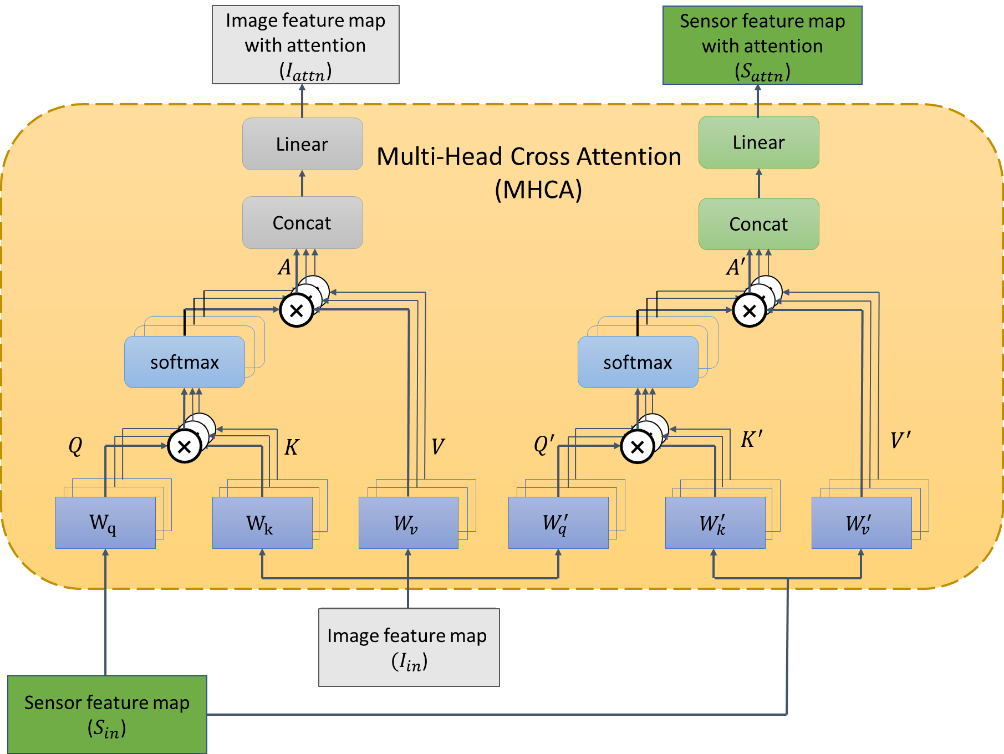
\includegraphics[width=0.8\linewidth]{pic/cross_attention.png}
  \caption{The Multi-Head Cross Attention Module (MHCA) structure serves as a central component of the Transformer Encoder for Fusion. It operates by taking in both the image feature map (\begin{math}
    I_{in}
  \end{math}) and the sensor feature map (\begin{math}
    S_{in}
  \end{math}) as inputs. The module employs cross-attention mechanisms to investigate the interrelationships and associations among each feature map and between the two feature maps. Through this approach, the MHCA module achieves an improved ability to identify meaningful features from both modalities, generating an image feature map with attention (\begin{math}
    I_{attn}
  \end{math}) and a sensor feature map with attention (\begin{math}
    S_{attn}
  \end{math}) as outputs.}
  \Description{Cross attention module in transformer.}
  \label{cross_attention}
\end{figure}

The Cross Attention module is proposed to model intra-modality relationships for image and sensor features. The structure of MHCA is shown in Figure \ref{cross_attention}. There are two branches to determine the parameters Query(\begin{math}
  Q
\end{math}, \begin{math}
  Q^\prime
\end{math}), Key(\begin{math}
  K
\end{math}, \begin{math}
  K^\prime
\end{math}), and Value (\begin{math}
  V
\end{math}, \begin{math}
  V^\prime
\end{math}). One branch calculates \begin{math}
  Q
\end{math}, \begin{math}
  K
\end{math}, \begin{math}
  V
\end{math} for Image feature map with attention \begin{math}
  I_{attn}
\end{math}. The other calculates \begin{math}
  Q^\prime
\end{math},\begin{math}
  K^\prime
\end{math},\begin{math}
  V^\prime
\end{math} for Sensor feature map with attention \begin{math}
  S_{attn}
\end{math}. The calculation process is given as followings:

\begin{equation}
  Q=S_{in}W_q,K=I_{in}W_k,V=I_{in}W_v
\end{equation}
\begin{equation}
  A=softmax\left(\frac{QK^T}{\sqrt{C/h}}\right)\ V
\end{equation}

\begin{equation}
  Q^\prime=I_{in}W_q^\prime,K^\prime=S_{in}W_k^\prime,V^\prime=S_{in}W_v^\prime
\end{equation}
\begin{equation}
  A^\prime=softmax\left(\frac{Q^\prime K^{\prime T}}{\sqrt{C/h}}\right)V^\prime
\end{equation}



where  \begin{math}
  W_q,W_k,W_v,W_q^\prime, W_k^\prime, W_k^\prime \in \mathbb{R}^{C\times\left(C/h\right)}
\end{math} are linear transformation matrix with learnable parameters. These Multiple matrixes are computed by multi-head.  C and h are the embedding dimension and number of heads, respectively. A and \begin{math}
  A^\prime
\end{math} are results of equation 6 and equation 8, respectively. Multiple A and \begin{math}
  A^\prime
\end{math} are concatenated, respectively. The sensor feature map \begin{math}
  S_{in}
\end{math} for one branch is used for query \begin{math}
  Q
\end{math} to compute \begin{math}
  K^\prime
\end{math} and then update \begin{math}
  V^\prime
\end{math}. The Image Feature Map \begin{math}
  I_{in}
\end{math} for another branch is used for query \begin{math}
  Q^\prime
\end{math} to compute key \begin{math}
  K
\end{math} and value \begin{math}
  V
\end{math}. Therefore, these two branches exchanges information between sensor and image features for sematic information sharing. The computation complexity of generating the attention map in cross-attention are linear rather than quadratic as in all-attention. The entire process for MHCA module is more efficient. And it can reduce the risk of overfitting.


\subsection{Loss function}
The leaf area index (LAI) data was manually collected from the farm and used as labels for the ViST model. Following data normalization, LAI values were scaled to a range of [0,1]. The loss function quantifies the discrepancy between the model's predicted value \begin{math}
  y^\prime
\end{math} and the actual value \begin{math}
  y
\end{math}. This non-negative, real-valued function is typically expressed as \begin{math}
  L(y, y^\prime)
\end{math} and serves as the foundation for the empirical risk function and the structural risk function.

In this paper, we approach crop growth prediction as a regression problem. A neural network with a single output node is typically used to solve regression problems, with the output value representing the predicted value. To evaluate the performance of our model, we use the mean square error loss function as the primary metric.

\begin{equation}
  MSE\left(y,y^\prime\right)=\frac{\sum_{i=1}^{n}\left(y_i-y_i^\prime\right)^2}{n}
\end{equation}

where \begin{math}
  n
\end{math} is the number of samples, \begin{math}
  y_i
\end{math} is the true value of the leaf area index for the i-th sample, and \begin{math}
  y_i^\prime
\end{math} is the predicted value of the leaf area index for the i-th sample. The MSE serves as a measure of the accuracy of our model’s output and is used to update the model parameters in subsequent iterations.

\section{Experiments and Results}

In this section, we will present the methods used for data collection, describe the equipment and data format employed. Following data collection, both image and sensor data undergo preprocessing. The evaluation criteria for model performance and experimental details will also be outlined.


\subsection{Data collection}

\begin{figure}[htbp]
  \centering
  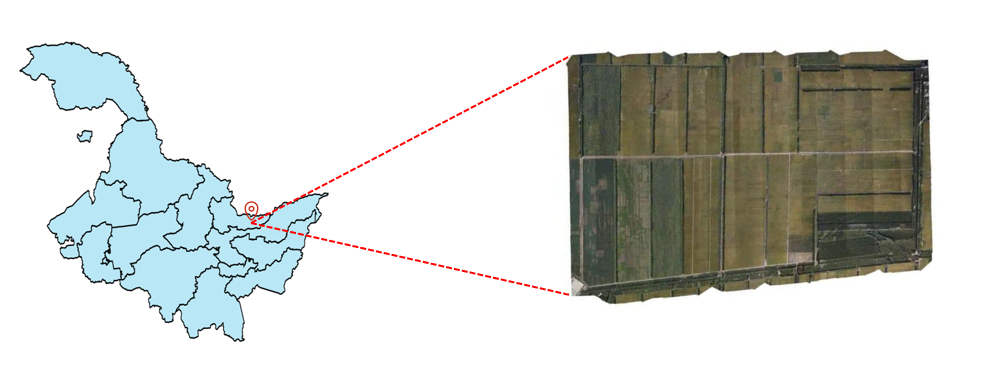
\includegraphics[width=\linewidth]{pic/farm_location.png}
  \caption{The data were collected at Farm 290, located in Suibin County, Hegang City, Heilongjiang Province, China.}
  \Description{Data collection farm location.}
  \label{farm_location}
\end{figure}


\begin{figure}[htbp]
  \centering
  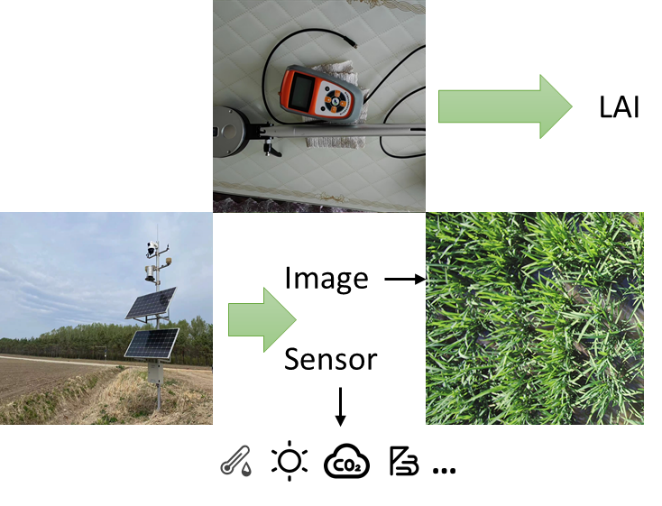
\includegraphics[width=0.5\linewidth]{pic/data_acquisition_equipment.png}
  \caption{Data acquisition equipment. The image and sensor data collection device is shown on the left, the leaf area index data collection device is shown in the middle, and image data is shown on the right.}
  \Description{Data acquisition equipment.}
  \label{data_collection_equipment}
\end{figure}


\begin{figure}[htbp]
  \centering
  \subcaptionbox{Rice image data.}{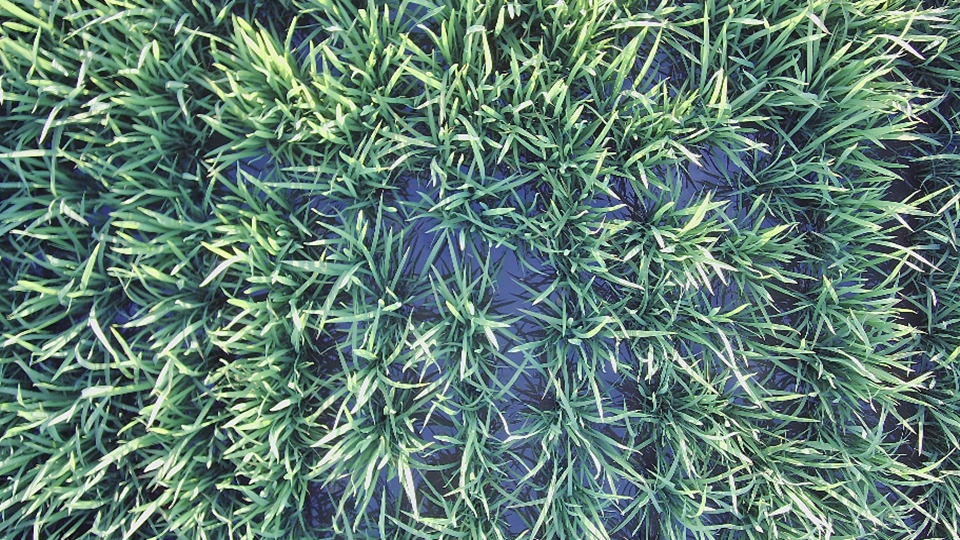
\includegraphics[width = 0.33\textwidth]{pic/rice.png}}
  \subcaptionbox{Soybean image data.}{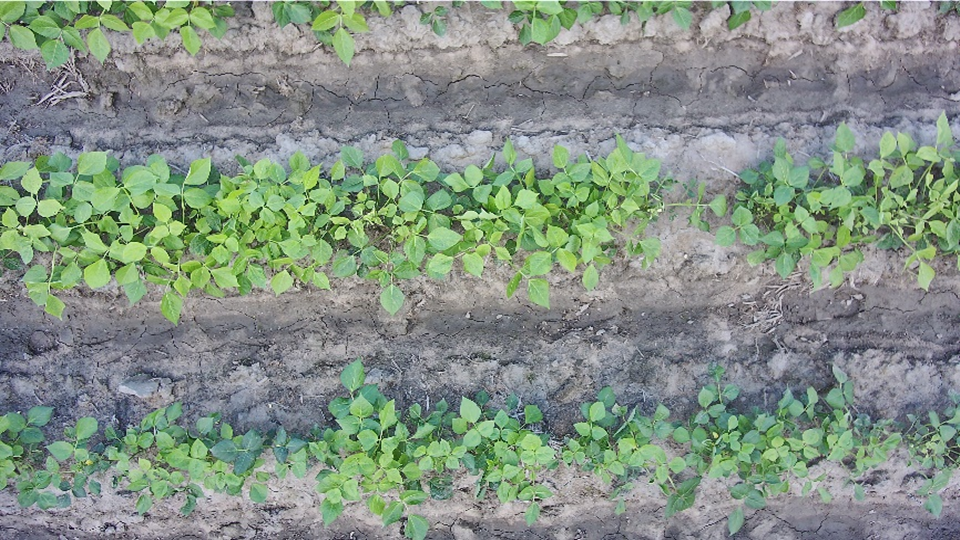
\includegraphics[width = 0.33\textwidth]{pic/soybean.png}}
  \subcaptionbox{Maize image data.}{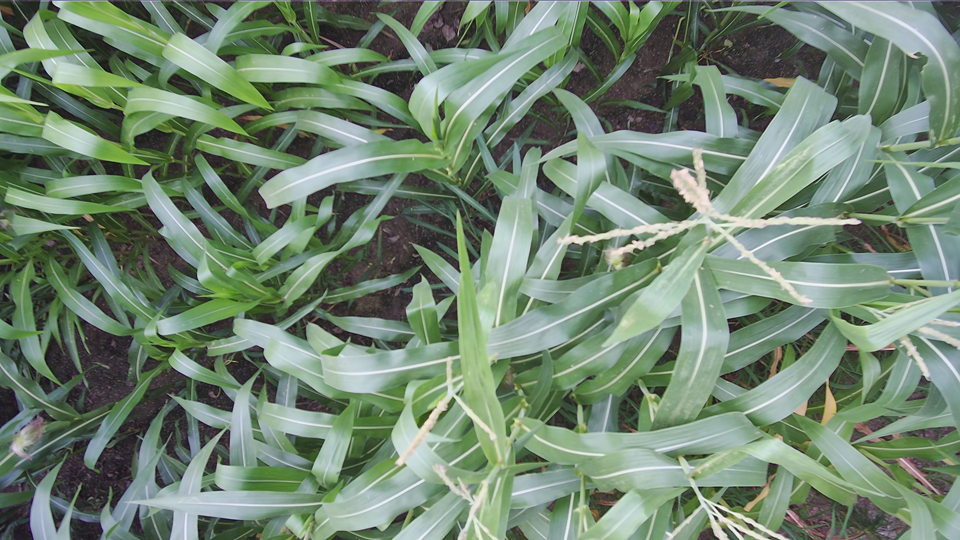
\includegraphics[width = 0.33\textwidth]{pic/corn.png}}\hfill
  % 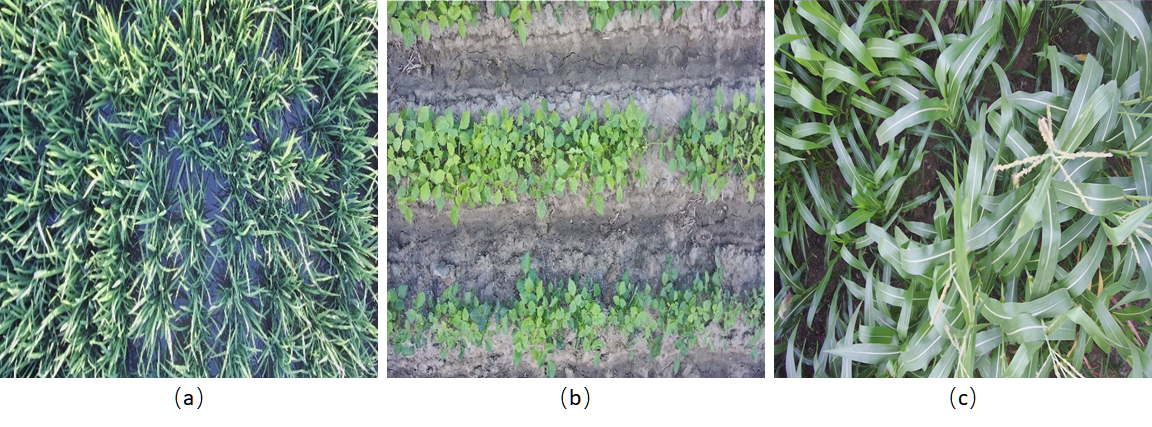
\includegraphics[width=\linewidth]{pic/crop.png}
  \caption{Crop image data.}
  \Description{Crop image data.}
  \label{crop}
\end{figure}

The location for data acquisition is shown in Figure \ref{farm_location}. The rice, maize, and soybean data were collected on farm. There are three sample points for each crop. There are totally 9 sample points on farm. The data acquisition device is shown in Figure \ref{data_collection_equipment}. One device placed at each sample point on farm includes one camera and 11 number of sensors. LAI data were collected periodically using a hand-held device at each sample point for data alignment.


The crops are photographed from a top view. The images of rice, soybeans, and maize captured by the camera on the farm are shown in Figure \ref{crop}(a)(b)(c), respectively. The height is set at 3 meters. The image format is RGB with a resolution of 3840×2160. The time interval between each image was two hours.


The collected items of sensors are shown in Table \ref{tab:sensor_and_data_items}, including eleven sensor data types. The soil sensors are deployed in the ground at 10cm, 20cm, 30cm, 40cm, and 50cm depths, respectively. Air, light, and Wind sensors are deployed on the top of the IoT Device. The time interval of data collection for each sensor is half an hour. The image and sensor data were collected and uploaded to the cloud server periodically for storage and data analysis.



\begin{table*}
  \caption{Sensor data. The table lists the data items captured by the sensors and their corresponding units.}
  \label{tab:sensor_and_data_items}
  \begin{tabular}{ll}
    \hline
    Data item        & Unit              \\
    \hline
    Carbon dioxide   & PPM               \\
    Soil temperature & Celsius           \\
    Soil humidity    & \%                \\
    Air temperature  & Celsius           \\
    Air humidity     & \%                \\
    Light intensity  & Klux              \\
    Wind direction   & degree            \\
    Wind speed       & Meters per second \\
    Air pressure     & Hpa               \\
    PM10             & PPM               \\
    PM2.5            & PPM               \\
    \hline
  \end{tabular}%
\end{table*}

\subsection{Data preprocessing}
\textbf{Preprocessing of image data:}To ensure better convergence in backpropagation, the image data was normalized to a specific range using the Z-score method on each image's data.

\begin{equation}
  z=\frac{x-\mu}{\sigma}
\end{equation}
In this study, where \begin{math}
  \mu
\end{math} denotes the mean value, \begin{math}
  \sigma
\end{math} represents the standard deviation, \begin{math}
  x
\end{math} denotes the input data, and \begin{math}
  z
\end{math} denotes the output data. The mean and standard deviation of the three channels of the image were recorded, respectively. Specifically, the mean value of the normalized image was set to 0 on each channel, and the variance was set to 1. However, it should be noted that this normalization method may not be applicable to cases with small sample sizes, and is generally recommended to be used only when the sample size exceeds 30. Table \ref{tab:image_standardized_data} presents the normalized results of image calculation for rice, soybean, and maize.

\begin{table}[htbp]
  \caption{Image standardized data. The table presents the mean and standard deviation values for the RGB channels of the images of three crops, namely rice, soybean, and corn. These values were obtained through the normalization process described in the previous section.}
  \label{tab:image_standardized_data}
  \begin{tabular}{lllc}
    \toprule
    crop                                            & channel   & mean   & standard deviation \\
    \midrule
    \multicolumn{1}{c}{\multirow{3}[1]{*}{rice}}    & Channel 1 & 0.4452 & 0.1973             \\
                                                    & Channel 2 & 0.5014 & 0.2035             \\
                                                    & Channel 3 & 0.4292 & 0.183              \\
    \midrule
    \multicolumn{1}{c}{\multirow{3}[0]{*}{soybean}} & Channel 1 & 0.5    & 0.1517             \\
                                                    & Channel 2 & 0.5355 & 0.1641             \\
                                                    & Channel 3 & 0.487  & 0.1497             \\
    \midrule
    \multicolumn{1}{c}{\multirow{3}[1]{*}{corn}}    & Channel 1 & 0.4452 & 0.1973             \\
                                                    & Channel 2 & 0.5014 & 0.2035             \\
                                                    & Channel 3 & 0.4292 & 0.183              \\
    \bottomrule
  \end{tabular}
\end{table}

\textbf{Preprocessing of sensor data:}To eliminate the influence of dimensions, we normalized each size using the following equation, as the numerical differences between dimensions in the sensor data were relatively large.



\begin{equation}
  x_{normalized} = \frac{x - x_{min}}{x_{max} - x_{min}}
\end{equation}

where \begin{math}
  x_{min}
\end{math} is the minimum value, and \begin{math}
  x_{max}
\end{math} is the maximum value. \begin{math}
  x_{normalized}
\end{math} is the normalized value.

The maximum and minimum values for each metric were saved in a separate file for data preprocessing when they were used for processing actual data. The processed data are shown in Table \ref{tab:sensor_input_metrics_preprocessing}.

\begin{table*}
  \caption{Sensor input metrics preprocessing. The table includes the indicators for sensor data processing, as well as their maximum and minimum values. \label{tab:sensor_input_metrics_preprocessing}}

  \begin{tabular}{lll}
    \hline
    \multicolumn{1}{l}{Indicators}            & \multicolumn{1}{l}{Minimum} & \multicolumn{1}{l}{Maximum} \\
    \hline
    Carbon dioxide                            & 364                         & 636                         \\
    Soil temperature for 10 centimeters depth & 18.1                        & 25.1                        \\
    Soil temperature for 20 centimeters depth & 18.3                        & 23                          \\
    Soil temperature for 30 centimeters depth & 18.3                        & 22.1                        \\
    Soil temperature for 40 centimeters depth & -30                         & -30                         \\
    Soil temperature for 50 centimeters depth & 17.1                        & 21.2                        \\
    Soil humidity for 10 centimeters depth    & 46.8                        & 80.6                        \\
    Soil humidity for 20 centimeters depth    & 53                          & 75.6                        \\
    Soil humidity for 30 centimeters depth    & 55.2                        & 79.5                        \\
    Soil humidity for 40 centimeters depth    & 0                           & 80.6                        \\
    Soil humidity for 50 centimeters depth    & 67.3                        & 81.5                        \\
    Air humidity                              & 31                          & 98.53                       \\
    PM10                                      & 0                           & 128                         \\
    PM2.5                                     & 0                           & 55                          \\
    Air pressure                              & 981.1                       & 1005.1                      \\
    Light intensity                           & 0                           & 200                         \\
    Air temperature                           & 16.37                       & 30.99                       \\
    Wind direction                            & 0                           & 359.8                       \\
    Wind speed                                & 0                           & 6.68                        \\
    LAI                                       & 1.3075                      & 1.91                        \\
    \hline
  \end{tabular}%
\end{table*}


\textbf{Processing of LAI data:}In order to ensure better convergence in backpropagation, the image data were normalized to a specific range using the Z-score method. For each crop, three sets of image and sensor devices were placed at the same position as the camera when measuring the LAI.  During the collection of LAI data, hand-held devices capture a part of areas covered by the camera device. LAI data were collected every 5 days. In order to obtain more data, the piecewise cubic Hermite interpolation polynomial (PCHIP) method was used, as described by Fritsch and Carlson \cite{fritsch1980monotone}. LAI data were available for each day and were interpolated for three sample points of rice, soybean, and maize as shown in Figure \ref{lai}(a),(b),(c), respectively. The left side of the figure shows the original data and the right side shows the interpolated data. The interpolated data appear smoother, as can be seen from the curves.

\begin{figure}[htbp]
  \centering
  \subcaptionbox{Before and after rice LAI interpolation \label{1}}{  \begin{minipage}{0.49\linewidth}
      \centering
      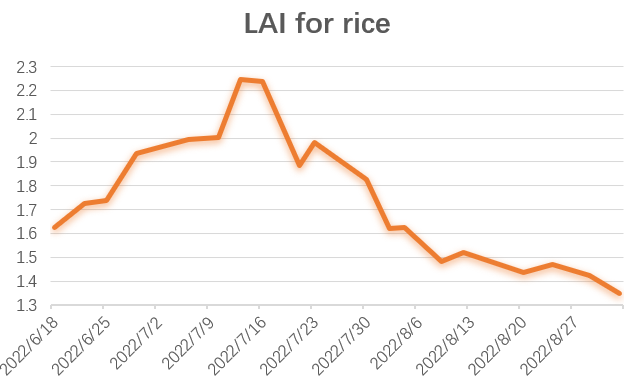
\includegraphics[width=\linewidth]{pic/rice_lai_before.png}
    \end{minipage}
    %\qquad
    \centering
    \begin{minipage}{0.49\linewidth}
      \centering
      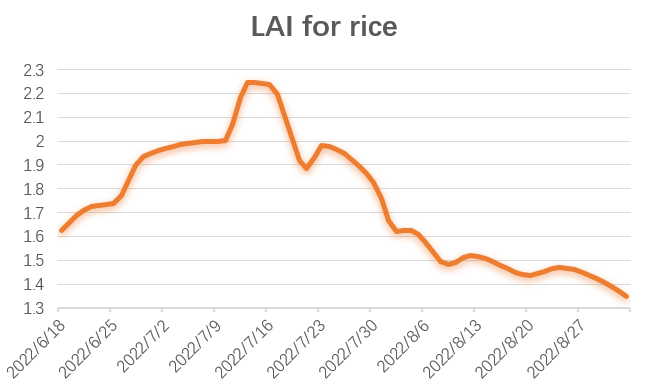
\includegraphics[width=\linewidth]{pic/rice_lai_after.png}
    \end{minipage}}\hfill

  \subcaptionbox{Before and after soybean LAI interpolation \label{2}}{  \begin{minipage}{0.49\linewidth}
      \centering
      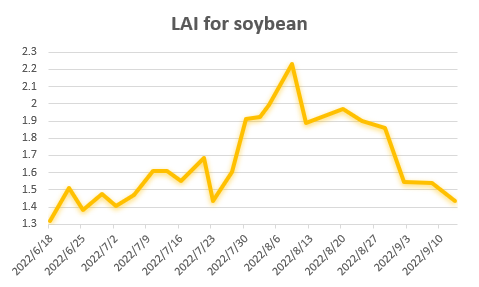
\includegraphics[width=\linewidth]{pic/soybean_lai_before.png}
    \end{minipage}
    %\qquad
    \centering
    \begin{minipage}{0.49\linewidth}
      \centering
      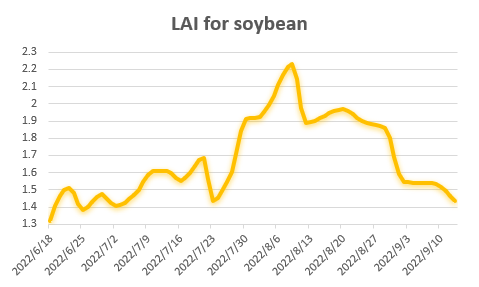
\includegraphics[width=\linewidth]{pic/soybean_lai_afterg.png}
    \end{minipage}}\hfill


  \subcaptionbox{Before and after maize LAI interpolation \label{3}}{  \begin{minipage}{0.49\linewidth}
      \centering
      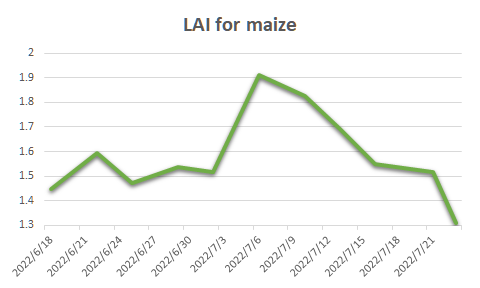
\includegraphics[width=\linewidth]{pic/corn_lai_before.png}
    \end{minipage}
    %\qquad
    \centering
    \begin{minipage}{0.49\linewidth}
      \centering
      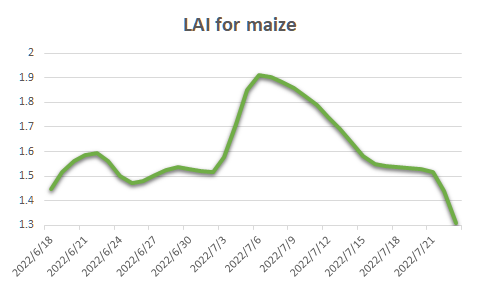
\includegraphics[width=\linewidth]{pic/corn_lai_after.png}
    \end{minipage}}\hfill
  \caption{LAI data preprocessing. The figure shows the leaf area index data before and after interpolation. The horizontal axis represents time, and the vertical axis represents the leaf area index.}
  \Description{LAI data preprocessing.}
  \label{lai}
\end{figure}



\textbf{Data alignment:} One sample includes image data, sensor data, and a label -- LAI data. The image data, sensor data, and LAI data were aligned based on their respective sampling location and time. Each image was captured at a two-hour interval, while the sensors' sampling frequency was every half hour. The time alignment between the data sets was established on a half-hour basis. Due to the smaller quantity of image data relative to the sensor data, four samples collected over a two-hour period corresponded to a single image. Notably, there is only one LAI data point per day; this means that forty-eight samples share the same LAI label.


\textbf{Training and test sets:}For each crop, three sample points were selected, yielding a total of nine observation points on the farm. Two of the sample points were utilized for model training, while the remaining sample point was used for model testing. Cross-validation was carried out across different sample points for each crop to prevent the problem of using the same sample data for both training and testing, which could result in a smaller difference in the data gradient.

The amount of data utilized in the experiment is illustrated in Fig. \ref{dataset_size}, with "days" denoting the duration of data collection. "Train sample" and "Test sample" refer to the number of data instances employed for training and testing, respectively.


\begin{table}[htbp]
  \centering
  \caption{The quantity of experimental data.}
    \begin{tabular}{llll}
    \toprule
    Crop  & Days & Train sample & Test sample \\
    \midrule
    Rice  & 83    & 7968  & 3984 \\
    Soybean & 87    & 8352  & 4176 \\
    Maize & 83    & 7968  & 3984 \\
    \bottomrule
    \end{tabular}%
  \label{dataset_size}%
\end{table}%


\subsection{Evaluation Metrics}
Mean square error (MSE), mean Absolute error (MAE), Mean Absolute Percentage Error(MAPE) and Symmetric Mean Absolute Percentage Error(SMAPE) are used to predict the performance of various models. MSE is the same as the loss function. MAE is the sum of the absolute differences between the target and prediction values.


\begin{equation}
  MAE=\frac{\sum_{i}^{n}\left|y_i-y_i^\prime\right|}{n} \label{mae}
\end{equation}

where \begin{math}
  y_i^\prime
\end{math} is the evaluated value of the model, \begin{math}
  y_i
\end{math} is the real value, and \begin{math}
  n
\end{math} is the total number of samples.

The Mean Square Error (MSE) is the mean of the squared differences between the model's evaluated value, and the actual sample value \begin{math}
  y
\end{math}. The formula is as follows:

\begin{equation}
  MSE=\frac{\sum_{i=1}^{n}\left(y_i^\prime-y_i\right)^2}{n} \label{mse}
\end{equation}

where \begin{math}
  y_i
\end{math} and \begin{math}
  y_i^\prime
\end{math},i are the true value and the corresponding evaluated value for the first sample, and \begin{math}
  n
\end{math} is the number of samples.

MAPE is a commonly used performance metric in estimation. It measures the accuracy of a estimation by calculating the absolute percentage difference between the estimation value \begin{math}
  y_i^\prime
\end{math} the actual value \begin{math}
  y_i
\end{math}, and then take the average of all the absolute percentage differences. The formula for calculating MAPE is as follows:

\begin{equation}
  MAPE=\frac{100\%}{n}\sum_{i=1}^{n}\left|\frac{y_i^\prime-y_i}{y_i}\right| \label{mape}
\end{equation}

where \begin{math}
  n
\end{math} is the number of samples, \begin{math}
  y_i
\end{math} is the actual value, and \begin{math}
  y_i^\prime
\end{math} is the estimate value.

SMAPE is a widely used metric for evaluating the accuracy of forecasting models. It is a symmetric error that calculates the average percentage difference between the actual and evaluated values . Unlike other error measures, SMAPE takes into account the magnitude of the actual values, making it a more reliable metric for comparing the accuracy of different forecasting models. The formula for calculating SMAPE is as follows:

\begin{equation}
  SMAPE=\frac{100\%}{n}\sum_{i=1}^{n}\frac{\left|y_i^\prime-y_i\right|}{\left(\left|y_i^\prime\right|+\left|y_i\right|\right)/2} \label{smape}
\end{equation}

where \begin{math}
  n
\end{math}, \begin{math}
  y_i
\end{math} and \begin{math}
  y_i^\prime
\end{math} are same as the symbols in MAPE formula. SMAPE ranges from 0\% to 200\%, with lower values indicating better accuracy.


\subsection{Experiments and results}

In this section, we present the extensive experiments conducted to demonstrate the effectiveness of our proposed ViST over existing methods. Our model was compared with the state-of-the-art models, such as Rice-Fusion \cite{9672157}, Rice-Transformer \cite{9864182}, CNN-Transformer \cite{8999620}, DNNF1, and DNNF2 \cite{maimaitijiang_soybean_2020}. While both DNNF1 and DNNF2 are multimodal models developed for soybean yield prediction, Rice-Fusion and Rice-Transformer employ multimodal approaches to diagnose rice diseases. The CNN-Transformer model was proposed to classify crops based on multitemporal data. In terms of comparison, the input and output to these models were kept the same as for our ViST model. Finally, the output of all models was evaluated based on the LAI value representing the crop growth status.

ViST was subjected to ablation studies with regards to its input modes, including image-only data, sensor-only data, and multimodality data. The performance of each model was evaluated using a range of metrics, including MAE, MSE, MAPE, and SMAPE which are presented in Equations \ref{mae},\ref{mse},\ref{mape}, and \ref{smape}, respectively.

The preprocessed data were utilized to train each model using the primary hyperparameters of ViST, which are outlined in Table \ref{tab:hyperparameters}. An Adam optimizer was employed, with a weight decay of 0.0001, and all models were trained on a GeForce RTX 3090 GPU. To dynamically adjust the learning rate, the cosine annealing strategy was implemented. The maximum number of iterations was determined based on the sample size and epoch, resulting in a monotonically decreasing learning rate with increasing epochs during the training process. The ViST model's primary hyperparameters can also be found in Table \ref{tab:hyperparameters}. Random normal distribution was used to initialize the parameters of each model. For the ablation experiment, the MM, SMI, and SMS were used as inputs for the model.



\begin{table}[htbp]
  \centering
  \caption{Main hyperparameters of the model.}
  \begin{tabular}{ll}
    \toprule
    Parameter     & \multicolumn{1}{l}{Parameter size} \\
    \midrule
    hidden size   & 768                                \\
    head num      & 12                                 \\
    layer num     & 12                                 \\
    MLP ratio     & 4                                  \\
    drop rate     & 0.1                                \\
    sensor num    & 19                                 \\
    epoch         & 50                                 \\
    batch size    & 32                                 \\
    weight decay  & 0.0001                             \\
    learning rate & 0.0001                             \\

    \bottomrule
  \end{tabular}%
  \label{tab:hyperparameters}%
\end{table}%

\subsubsection{Experiments and results for a single crop}


In this section, we evaluated the performance of our model on three crops - rice, soybean, and maize. Firstly, we compared the model's performance using single modality data and multimodality data, as discussed in Section A. Secondly, we compared the performance of our ViST model with that of other models, as outlined in Section B.

\textbf{A.Performance Comparison of ViST model with single modality data and multimodality data}	

The ViST model was trained for each crop with three different data input modes: image data, sensor data, both of image and sensor data. Thus, three trained models were obtained for each crop.

\begin{table}[htbp]
  \centering
  \caption{ViST model test results for different input modes.}
    \begin{tabular}{llllll}
    \toprule
    Crop  & \multicolumn{1}{l}{Input mode} & MSE   & \multicolumn{1}{l}{MAE} & MAPE  & SMAPE \\
    \midrule
    \multirow{3}[1]{*}{rice} & Sensor & \textbf{0.00227} & 0.03469 & 0.14928 & 13.1395 \\
          & Image & 0.00548 & 0.0527 & 0.27484 & 20.19456 \\
          & Multimodality & 0.00244 & \textbf{0.01344} & \textbf{0.05614} & \textbf{5.26049} \\
          \midrule
    \multirow{3}[0]{*}{soybean} & Sensor & 0.03201 & 0.12261 & 0.67907 & 34.33472 \\
          & Image & 0.00536 & 0.04973 & 0.31889 & 15.41658 \\
          & Multimodality & \textbf{0.00007} & \textbf{0.00351} & \textbf{0.02644} & \textbf{2.06496} \\
          \midrule
    \multirow{3}[1]{*}{maize} & Sensor & 0.00183 & 0.03185 & 0.14455 & 12.50781 \\
          & Image & 0.00409 & 0.04577 & 0.19804 & 13.61606 \\
          & Multimodality & \textbf{0.00003} & \textbf{0.00304} & \textbf{0.01768} & \textbf{1.53183} \\
    \bottomrule
    \end{tabular}%
  \label{tab:vist_model_test_results}%2
\end{table}%


After the trained models were obtained, we used the data from the test dataset to test the models. The performance of the ViST model for test dataset is shown in table \ref{tab:vist_model_test_results}.

It is shown that the multimodality mode has achieved the lowest value of the prediction indictors among three modes for three crops. As four indictors have shown the same trend on the experiment results, MAE is used to analysis the performance of the ViST model. In the rice experiment, the value of MAE decreases by, 61.25\%, 74.49\% compared to that of the sensor and image mode, respectively. In the soybean experiment, the value of MAE decreases by 97.13\%, 92.94\%, compared to that of the sensor and image mode, respectively. In the maize experiment, the value of MAE decreases by 90.45\%, 93.35\%, compared to that of the sensor and image mode, respectively. Therefore, it can be concluded that combining image and sensor data significantly improves the performance for ViST model. And both sensor and image data have almost equal contribution for model training.

For rice, sensors are more effective than images because there is little difference in rice images during growth and leaf features are not prominent. For soybeans, images are more effective than sensors because the image features change significantly during growth. There is little difference between image and sensor data for corn, and both are effective in reflecting crop growth because error rates for various evaluation indices are relatively small. 

Using image analysis, crop surface texture features, such as color, texture, and shape, can be analyzed to infer the healthy status of the crop, including whether it is growing well and whether it is affected by pests and diseases. Sensor data can capture changes in environmental factors, such as temperature, humidity, light, and soil, to assess their impact on crop growth. For example, excessive drought or excessive moisture can have a negative effect on crop growth. By comprehensively analyzing these two aspects of information, crop growth can be more accurately evaluated, and appropriate agricultural management measures can be adjusted accordingly. 

In the experiments on rice, soybeans, and corn, the multi-modality results were better than the single-modality results. Multi-modal data can supplement the information that is lacking in single-modality data, completing the information gap. For example, images only reflect surface information of the crop, while sensors only reflect environmental information. If only single modality data is used, many important pieces of information will be ignored. By integrating multiple types of information, different types of information can complement each other, improving the accuracy and comprehensiveness of data analysis. 

The fusion of image and sensor multi-modal data can complete noise suppression. Noise on the data is common, especially in sensor data processing. However, multi-modal data can reduce noise on the data by fusing the data, which is more robust than single modality data analysis. 

Single-modality data is more susceptible to interference than multi-modality data, which is more robust. Sensor data is often affected by various external environmental factors (such as rain, dust, and occlusion), which can affect data accuracy. Conversely, image data is less affected by external factors. Therefore, in multi-modality data analysis, the combination of image data significantly improves data accuracy and robustness. 

Thus, the complementary nature, noise suppression, and robustness of multi-modal data analysis can more comprehensively understand things’ essence and more accurately describe the actual situation.




\textbf{B.Comparison with other models}

In this Section, we compared the proposed ViST model with other models: DNNF1, DNNF2, CNN-Transformer, Rice-Fusion, Rice-Transformer . All three models were trained on rice, soybean, and maize data, respectively.

% Table generated by Excel2LaTeX from sheet 'Sheet1'
\begin{table}[htbp]
  \centering
  \caption{The comparative experimental test results of rice.}
    \begin{tabular}{lllll}
    \toprule
    Model & MSE   & MAE   & MAPE  & SMAPE \\
    \midrule
    CNN-Transformer & 0.00024 & 0.01368 & 0.04287 & 4.3371 \\
    DNNF1 & 0.00177 & 0.01775 & 0.08548 & 7.21533 \\
    DNNF2 & 0.00333 & 0.02816 & 0.11206 & 10.303 \\
    Rice-Fusion & 0.00024 & 0.01065 & 0.04215 & 3.95636 \\
    Rice-Transformer & 0.00244 & 0.01344 & 0.05614 & 5.26049 \\
    ViST  & \textbf{0.00023} & \textbf{0.00923} & \textbf{0.03263} & \textbf{3.15724} \\
    \bottomrule
    \end{tabular}%
  \label{rice_results}
\end{table}%

Table \ref{rice_results} shows the experimental results of various models when applied to the rice dataset. The ViST model showed the best performance on all prediction metrics, implying its excellent performance in estimating rice growth. In the average, ViST lowered MSE by 55.80\%, MAE by 38.48\%, MAPE by 44.21\%, and SMAPE by 42.59\%. Compared to the other models, the ViST model shows better performance in accuracy and stability, especially when compared to DNNF1 and DNNF2. For instance, compared to DNNF1, ViST lowered MSE by 87.01\%, MAE by 48.00\%, MAPE by 61.83\%, and SMAPE by 56.24\%. It is also shown that ViST has almost same value on MSE with CNN-Transformer and Rice-Fusion model.

% Table generated by Excel2LaTeX from sheet 'Sheet1'
\begin{table}[htbp]
  \centering
  \caption{The comparative experimental test results of soybean.}
    \begin{tabular}{lllll}
    \toprule
    Model & MSE & MAE & MAPE & SMAPE \\
    \midrule
    CNN-Transformer & 0.00013 & 0.00749 & 0.0705 & 3.43951 \\
    DNNF1 & 0.00016 & 0.00958 & 0.05863 & 4.10262 \\
    DNNF2 & 0.00091 & 0.01597 & 0.08465 & 6.45109 \\
    Rice-Fusion & 0.00018 & 0.00656 & 0.0969 & 3.74191 \\
    Rice-Transformer & 0.00014 & 0.00478 & 0.08859 & 3.17471 \\
    ViST  & \textbf{0.00007} & \textbf{0.00351} & \textbf{0.02644} & \textbf{2.06496} \\
    \bottomrule
    \end{tabular}%
  \label{soybean_results}%
\end{table}%

Similarly to Table \ref{rice_results}, Table \ref{soybean_results} presents the experimental results of ViST and other comparative models. The experiments in Table \ref{soybean_results} use soybean data as the dataset. By considering the improvement ratios relative to the other models, it is evident that ViST achieves significant enhancements across all four metrics, with the most notable improvements visible on the MAE and MAPE metrics. Regarding the MSE metric, ViST achieves reductions of 56.25\%, 92.31\%, 61.11\%, and 50.00\% compared to DNNF1, DNNF2, Rice-Fusion, and Rice-Transformer, respectively. Furthermore, ViST decreases the error by 46.15\% relative to CNN-Transformer.

% % Table generated by Excel2LaTeX from sheet 'Sheet1'
\begin{table}[htbp]
  \centering
  \caption{The comparative experimental test results of maize.}
    \begin{tabular}{lllll}
    \toprule
    Model & \multicolumn{1}{l}{MSE} & \multicolumn{1}{l}{MAE} & \multicolumn{1}{l}{MAPE} & \multicolumn{1}{l}{SMAPE} \\
    \midrule
    CNN-Transformer & 0.00013 & 0.00805 & 0.03245 & 4.27382 \\
    DNNF1 & 0.00026 & 0.00926 & 0.05208 & 4.83925 \\
    DNNF2 & 0.00009 & 0.00775 & 0.02958 & 3.10525 \\
    Rice-Fusion & 0.00007 & 0.00609 & 0.01712 & 1.71803 \\
    Rice-Transformer & 0.00012 & 0.00672 & 0.02436 & 2.39245 \\
    ViST  & \textbf{0.00003} & \textbf{0.00304} & \textbf{0.01768} & \textbf{1.53183} \\
    \bottomrule
    \end{tabular}%
  \label{tab:maize_results}%
\end{table}%


Table \ref{tab:maize_results} shows the experimental results of various models when applied to the maize dataset. The Rice-Fusion model exhibits good performance across four performance metrics, though slightly worse than ViST in terms of MAPE and SMAPE. Despite this, it still outperforms other models. The CNN-Transformer model demonstrates intermediate performance across the four metrics, slightly outperforming the DNNF1 and DNNF2 models with only small variations. It is apparent that the ViST model exhibits a reduction in error percentages greater than 50\% for both MAE and MSE metrics. This suggests that the ViST model is able to more accurately predict experimental data and is more stable and reliable in comparison to other models.

The result for three crops compared with other models indicates that the visual and spatiotemporal information captured by ViST is critical in estimating rice growth accurately. Cross attention mechanics can effectively extract texture from leaf image and fusion sensor data with image feature.  This suggests that the ViST model is able to more accurately evaluate experimental data and is more stable and reliable in comparison to other models.

\subsubsection{Experiments and results for combined data training}

% Table generated by Excel2LaTeX from sheet 'Sheet1'
\begin{table}[htbp]
  \centering
  \caption{The comparative experimental test results for hybrid.}
    \begin{tabular}{lllll}
    \toprule
    Model & \multicolumn{1}{l}{MSE} & \multicolumn{1}{l}{MAE} & \multicolumn{1}{l}{MAPE} & \multicolumn{1}{l}{SMAPE} \\
    \midrule
    CNN-Transformer & 0.00019 & 0.00822 & 0.03928 & 2.994976 \\
    DNNF1 & 0.00141 & 0.01928 & 0.09484 & 7.311991 \\
    DNNF2 & 0.00083 & 0.01388 & 0.04452 & 4.104376 \\
    Rice-Fusion & 0.00024 & 0.00857 & 0.04541 & 3.579631 \\
    Rice-Transformer & 0.00038 & 0.00614 & 0.03564 & 2.467895 \\
    ViST  & \textbf{0.00014} & \textbf{0.00591} & \textbf{0.02775} & \textbf{2.408083} \\
    \bottomrule
    \end{tabular}%
  \label{tab:hybrid_results}%
\end{table}%

The data from three crops were combined and used to train the model to test the model's generalization ability for the growth prediction of multiple crops. If only a single crop dataset is used to train the model, the model will focus too much on the characteristics of that crop, increasing the risk of overfitting. However, training the model with multiple crop datasets can reduce the risk of overfitting and improve the model's stability. With the application of many artificial intelligence technologies, data in the field of agriculture has become very rich. However, the amount of data for each crop itself is not large. Therefore, training the model with multiple agricultural datasets can better utilize limited data resources and improve the model's applicability.Table \ref{tab:hybrid_results} shows the results of ViST, DNNF1, DNNF2, CNN-Transformer, Rice-Fusion, Rice-Transformer models with the hybrid data set. The ViST model outperforms other models, particularly in terms of MAPE and SMAPE with higher accuracy. ViST's MAE performance is superior to other models, showing a 28.10\%, 3.75\%, and 31.04\% reduction compared to the CNN-Transformer, Rice-Transformer, and Rice-Fusion models, respectively. Furthermore, ViST's outstanding performance in MSE indicates its ability to capture data features effectively, with reductions of 26.32\%, 63.16\%, and 41.47\% compared to the CNN-Transformer, Rice-Transformer, and Rice-Fusion models, respectively.

The cross-attention mechanism adopted in ViST can fuse information from input data better, thus improving model performance and generalization capability. The performance of DNNF1 and DNNF2 based on multi-layer perceptron is worst due to their lack of complexity and flexibility in model structure, resulting in ineffective handling of various crop growth estimation tasks compared to ViST.

% Table generated by Excel2LaTeX from sheet 'Sheet1'
\begin{table}[htbp]
  \centering
  \caption{Comparison Results of ViST model with different crops as input.}
    \begin{tabular}{llllll}
    \toprule
    Train data & \multicolumn{1}{l}{Test data} & \multicolumn{1}{l}{MSE} & \multicolumn{1}{l}{MAE} & \multicolumn{1}{l}{MAPE} & \multicolumn{1}{l}{SMAPE} \\
    \midrule
    Rice  & Rice  & 0.00244 & 0.01344 & 0.05614 & 5.26049 \\
    Soybean & Soybean & 0.00007 & 0.00351 & 0.02644 & 2.06496 \\
    Maize & Maize & \textbf{0.00003} & \textbf{0.00304} & \textbf{0.01768} & \textbf{1.53183} \\
    Three crops & Three crops & 0.00014 & 0.00591 & 0.02775 & 2.40808 \\
    \bottomrule
    \end{tabular}%
  \label{tab:ubiquitous}%
\end{table}%

The table presents the results of ViST for four sets of experiments involving rice, soybean, corn, and a mixture of the three crops data. The results on the ubiquitous ability of ViST are shown in Table \ref{tab:ubiquitous}. The model for Maize data exhibits relatively lower prediction errors compared to other crop data. For example, in terms of the SMAPE metric, the error value of maize is 1.53\%, while the error values of rice, soybean, and a mixture of three crops are 5.26\%, 2.06\%, and 2.41\%, respectively. It can be seen that maize shows better performance. The reason is that Maize has the most feature.

In the mixed experiment of the three crops, the error values of all prediction indicators are slightly increased relative to the single crop experiment, but the magnitude of the increase is small. This indicates that ViST exhibits a high level of prediction accuracy and robustness in handling multi-crop information, and therefore has high practical value for agricultural production applications. As training data is derived from various crops, inter-crop differences may exist and may affect the accuracy and stability of the model. The efficacy of combined training, with the exception of training with rice data, is comparatively suboptimal in contrast to that of other training with soybean and maize data.
\begin{figure}[h]
  \centering
  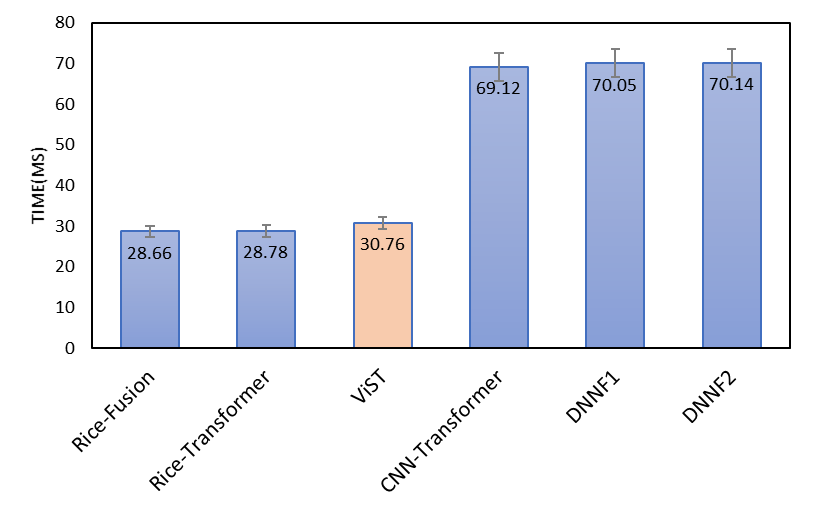
\includegraphics[width=0.6\linewidth]{pic/speed_test.png}
  \caption{Speed test results of the models.To compare the inference speed of models, each model performed 1000 inference runs, and the average result was taken as the final outcome. The horizontal axis represents the model name, and the vertical axis represents the average time for each inference run, in milliseconds. Each experimental result has an error rate of \begin{math}
    \pm
  \end{math}5\%.}
  \Description{Speed test results of the models.}
  \label{speed_test}
\end{figure}
\subsubsection{Experiments and results for speed test}



 From experimental results in Figure\ref{speed_test}, it is shown that the inference speed of ViST is much close to that of Rice-Fusion and Rice-Transformer. Compared to CNN-Transformer, DNNF1, and DNNF2, ViST's inference time is approximately 50\% of theirs. The CNN model requires more convolution operations, resulting in a relatively greater computational load and slower inference speeds. The multilayer perceptron model entails a larger number of parameters and computational load, leading to slower inference speeds. The performance of DNNF1 and DNNF2 based on multi-layer perceptron is worst due to their lack of complexity and flexibility in model structure, resulting in ineffective handling of various crop growth estimation tasks compared to ViST. Although DNNF1 and DNNF2 are simple, the fusion of images and sensors results in unsatisfactory performance.

\section{Conclusion and future directions}

This paper has proposed a Transformer-based ViST model for crop growth prediction by image and sensor data on a farm. The cross-attention mechanism in the model was used to improve the effect of model data fusion. The data of the three crops were trained together as input to the model. The model not only achieves high accuracy but also maintains a relatively fast speed. Experiment results show that the model with multimodality data can improve crop growth predication. Although the ViST model has achieved good results, there are still a number of limitations. As the model requires cross-modal feature fusion, this may increase the computational cost and training time of the model. And the ubiquitous of the model needs to be further validated in different crops to determine its applicability and generalizability. In the future, more crop growth data will be collected for model optimization. Furthermore, investigating the model's use in practical agricultural production can assist farmers in better decision-making and production management.









%%
%% The acknowledgments section is defined using the "acks" environment
%% (and NOT an unnumbered section). This ensures the proper
%% identification of the section in the article metadata, and the
%% consistent spelling of the heading.
\begin{acks}
  This research is supported by New generation artificial intelligent program, No.21ZD0110900 in CHINA, Heilongjiang NSF funding, No. LH202F022.
\end{acks}

%%
%% The next two lines define the bibliography style to be used, and
%% the bibliography file.
\bibliographystyle{ACM-Reference-Format}
\bibliography{sample-base}


%%
%% If your work has an appendix, this is the place to put it.
\appendix



\end{document}
\endinput
%%
%% End of file `sample-acmsmall.tex'.
